\documentclass{article}
\usepackage[a4paper, margin=2cm]{geometry}
\usepackage[utf8]{inputenc}
\usepackage{biblatex} % Bibliography
\usepackage{graphicx} % Figures
\usepackage{gensymb} % Mathematical symbols.
\usepackage{caption}
\usepackage{subcaption}
\usepackage{minted} % Code formatting
 

\title{Using Big Data time \& frequency domain analysis for optimal sensor fusion design}
\author{Dario Antonio Quintero Dominguez}
\date{\today}

% Bibliography
\bibliography{biblist.bib}

\begin{document}
\maketitle
\begin{abstract}
    Multi-dimensional Big Data analysis was performed to characterize and define the optimal configuration of a multi-sensor heading reference system. A complementary sensor system of a compass and gyro systems was analysed by varying their cutoff frequencies and simulation-time parameters with time-domain statistical analysis. Operational limitations for all components are described. The optimal cutoff frequency was selected at 1 $rad/s$ since this is the ""steady state" frequency after which all larger cutoff frequencies do not alter the response even when varying simulation time. A combination of standard deviation and RMS is suggested as the error metric for the sensors.
\end{abstract}

\section{Sensor Heading System}
% A5.1 Construct the complete heading system model in SIMULINK and include the diagram in your report. Also give details of the parameters used in the blocks representing the various subsystems. (10 marks)

The design of a heading directional sensor system is inherently related to the aircraft in which it is installed. Mechanical loads, vibrations, and operational frequencies interfere with electro-mechanical sensors and the outputted electronic signals accordingly. Small or medium sized UAVs also require a an independent heading system when telecommunication is not possible. The fundamental configuration of the integration of a gyroscope and a magnetic compass will be analysed for this scenario and optimal system design metrics are proposed. 

In order to design a low cost system, off-the-shelf components are selected. The magnetic compass is lightly damped due to fluid viscosity, and has a rise time $t_{rise} = 0.4s$ and settling time $t_{settling} = 18s$. Levi et al. \cite{levi2005gyro} describe how traditional magnetic compasses are subject to errors from both local magnetic fields and accelerations due to motion. These can also contribute to further dynamic controls.

% S4.1 Construct a model of a magnetic compass. Represent the compass as a second order system with unity sensitivity, rise time 0.4s and settling time 18s. The input to your compass model will be true heading and the output will be the heading indicated by the compass needle.

% ➢ S4.2 Produce a Bode plot (gain and phase frequency response) of the compass and use this to identify the useable frequency range of this sensor.
Given the step response parameters above, the compass system can be idealized as a second order system in the form of Equation \ref{eq:second_order_differential} in the time domain and Equation \ref{eq:second_order_transfer_function} in the Laplace domain as further where $w_n$ is natural frequency, $\zeta$ is the damping ratio, and $\lambda$ is the response amplitude gain described by \cite{ogata2010modern}. The under-damped equation condition of a damping ratio $\zeta << 1$ is tested and determined to be valid in Equation \ref{eq:second_order_damping_ratio_approximation}. The derived transfer function in Equation \ref{eq:second_order_transfer_function} can be analysed in MATLAB in the frequency domain using bode plots. It provides an indication of the response for several frequencies excitation as observed in Figure \ref{fig:compass_bode_plots}.

\begin{equation}
    \zeta \approx \frac{3}{w_n t_{settling}} 
\approx \frac{3 t_{rise}}{1.02 t_{settling}}
\approx 2.94 \frac{t_{rise}}{t_{settling}} = 0.0666
\label{eq:second_order_damping_ratio_approximation}
\end{equation}

%The 3dB cutoff maximum frequency is limited at a maximum slope of 0.12. The minimum and maximum safe operational frequency of the sensor is:  1.4969 rad/s with a maximum magnitude of 1 dB

\begin{equation}
\ddot{y}(t) +2 \zeta \dot{y} w_n (t) + w_n^2 y(t) = \lambda w_n^2 u(t)
\label{eq:second_order_differential}
\end{equation}

\begin{equation}
\frac{Y(s)}{U(s)} =
\frac{\lambda w^{2}_{n}}{s^2 + 2 \zeta w_n s + w^{2}_{n}} =
\frac{6.25}{s^2 + 0.333s + 6.25} 
\label{eq:second_order_transfer_function}
\end{equation}

Mathematically it is known from the bode plots that the compass system operates linearly at low mechanical frequencies. To analytically derive this linear range of the response below 3dB, the slopes between the plot sample points were taken to determine their limit closer to 0. All the green points within the magnitude analytic bode plot have a slope between the points of 0.15, and the maximum linear response at this position occurs at 1.29 $rad$ with a magnitude of 2.59 $dB$. If the linear slope restriction would be lowered to 0.12, for example, the maximum response in this line would be at the sampled point of 1.04 $rad$ with a maximum magnitude of 1.4969 $dB$. The frequency response of the compass becomes nonlinear since it has a resonance at the natural frequency $w_n$. The resonant point is achieved at 2.55 rad with a magnitude of 16.7 dB. The poles are derived as $p_{1,2} = \zeta w_n \pm jw_n\sqrt{1 - \zeta^2}$ for an under-damped system \cite{ogata2010modern} with the damping ratio approximation described in Equation \ref{eq:second_order_damping_ratio_approximation}. The two horizontal lines in Figure \ref{fig:compass_bode_plots} indicate the -3 $dB$ and + 3 $dB$ range of the response for amplification comparison reference. For the purposes of this sensor model, a transfer function block with these parameters is used in Simulink.

\begin{figure}
    \centering
    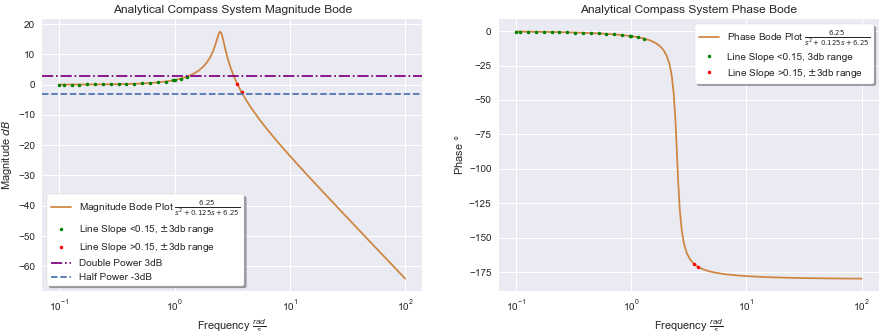
\includegraphics[width=\textwidth]{img/compass_bode_plots.png}
    \caption{Compass Bode Plot}
    \label{fig:compass_bode_plots}
\end{figure}

%S4.3 Construct a model of a gyro compass. Represent the gyro-compass as an ideal sensor with error modelled as integrated white noise with an offset, e.g. Fig. 8.
In order to accurately model the gyro, its mechanical operation needs to be considered. The physical design of a rate gyro is described in Morris \& Langari \cite{MORRIS2016599}, and consists of mainly consists of a spinning wheel attached to a gimbal rotational support that rotates around a fixed static frame of the sensor. The idealised physical behaviour of how this gyro is described in the time domain and Laplace domain is shown in Equation \ref{eq:gyro_transfer_function}. If the spinning mass is has large enough angular momentum $h$, it would mean that large, torques $T$ exerted on the sensor would force small rotation $\Theta_m$ that could be measured by a transducer. Assuming a burst of wind generates torques within the gyro frequency range, destabilizing friction, material stiffness and a limited measurement range could provide inaccurate signals. Hence, low turning rates might not be accurately measured, whereas higher turning rates would.

\begin{equation}
T(s) = {\mathcal {L}}\{h\dot{\theta_m}\} = sh\theta_m
\label{eq:gyro_transfer_function}
\end{equation}

\begin{equation}
\frac{\theta_m}{T} = \frac{1}{sh}
\end{equation}

To model these imperfections within Simulink, a random number with mean of 0.02 and standard deviation of 0.1 would be the equivalent of $\frac{1}{h}$ as observed in Figure \ref{fig:gyro_simulink_block}. A value for $h$ cannot be explicitly determined since this modelling includes random error considerations. This multiplies an integrator block $\frac{1}{s}$. Purely analytically, it is known that the bode plot of an integrator is a line with a negative slope as observed in Figure \ref{fig:gyro_bode}, and it would also have jitter when considering the random mean gain. A discrete Fast Fourier transform could also have performed on the integrator output to obtain this diagram. However, for the purposes of idealistic design, it can already be observed that for a range of frequencies of $10^{-2}$ to $10^{2}$ $rad/s$ the gyro system provides a linear magnitude response with attenuation at faster frequencies. After the $10^{2}$ $rad/s$ point, the gyro would not respond to higher frequencies.


\begin{figure}[H]
\begin{subfigure}{.4\linewidth}
  \centering
  % include first image
  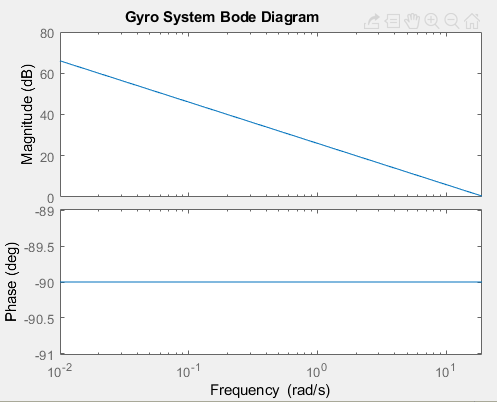
\includegraphics[width=\linewidth]{img/gyro_system_bode.PNG}  
  \caption{Gyro System Bode Plot}
  \label{fig:gyro_bode}
\end{subfigure}
\begin{subfigure}{.6\linewidth}
  \centering
  % include second image
  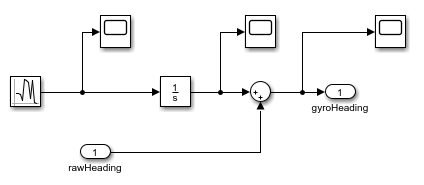
\includegraphics[width=\linewidth]{img/gyro_simulink_block.PNG}  
  \caption{Gyro Simulink block.}
  \label{fig:gyro_simulink_block}
\end{subfigure}
\caption{Gyro Simulink Bode}
\label{fig:fig}
\end{figure}


%➢ S4.4 Sketch the frequency spectrum of the output of the random number block, and the gain frequency response of an integrator, hence sketch the frequency spectrum of the error signal added to the true heading.

% ➢ S4.5 Suggest the useable frequency range of the gyro compass – note it is not possible to quantify in the same way as the magnetic compass

% S4.6 Determine the transfer functions for a pair of complementary first order filters with gain of ‘1’ in the pass band. Choose a suitable cut-off frequency for your filters based on the results of T4.2/T4.5. 
Fox et al. \cite{foxlin1996inertial} demonstrate how sensor fusion through complementary filters integrates responses to minimize individual sensor errors through Kalman algorithms. A simpler, non-probabilistic approach, will be tested by creating complementary filters with the mathematical relationship in Equation \ref{eq:complementary_filters} where the time constant $\tau = \frac{1}{w_{c}}$ is inverse to the cutoff frequency $w_{c}$ in $rad/s$. Since filters have the same cutoff frequency, when the low pass $L(s)$ compass filter response begins diminishing, the high pass $H(s)$ gyro filter magnitude increases. There is no amplification gain from this sensor configuration since its absolute value is unity ($K=1$). The optimal cutoff frequency would reduce the levels of oscillations of the full system signal by making each sensor respond within its ideal operational range. 

\begin{equation}
    L(s) + H(s) =
    \frac{s}{s + \frac{1}{\tau}} +  K{\frac  {1}{\tau s+1}} = 1
    \label{eq:complementary_filters}
\end{equation}



Using all the numerical parameters described previously, sensor fusion was performed and analysed on a magnetic compass and gyroscope as observed in Figure \ref{fig:simulink_model} using Simulink. The selected solver configuration was the variable step ODE-45 with 0.1 sample time was selected since it consistently provided expected results. Although larger sampling times also provided accurate results, computational efficiency was not completely needed for the algorithms in this model. The standard simulation time selected was 350 seconds.

\begin{figure}[h]
    \centering
    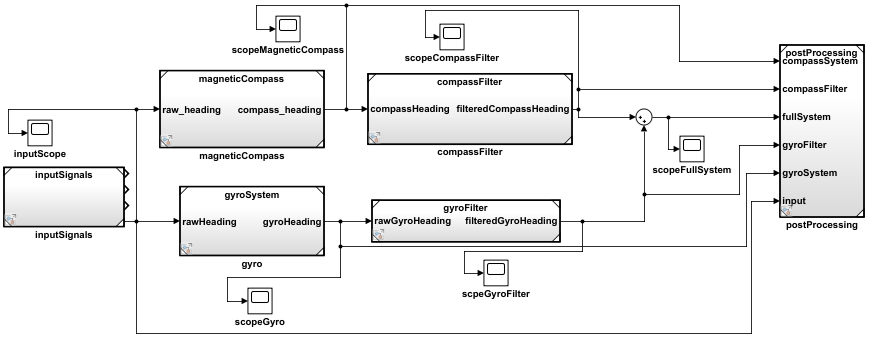
\includegraphics[width=\textwidth]{img/simulink_model.PNG}
    \caption{Heading system Simulink model}
    \label{fig:simulink_model}
\end{figure}

Several improvements could be done to this sensor fusion design to improve its accuracy, and possible future work could be performed analysing its behaviour. Within traditional aircraft navigation, once the rotational motion is negligible, the zero offset of the gyroscope is generally re-tuned, adding some degree of error. Micro-electrically modulated gyroscopes also reduce the zero-offset error, and Kalman auto-correction algorithms could be implemented as described by Levi et al. \cite{levi2005gyro} and Carque et al. \cite{carque2011sensor}. Integrating accelerometers into the heading system can further improve the accuracy of the signal since inertial changes can be considered alongside mobility changes of the gyro at higher frequencies; as described by Young Quist \cite{youngquist1997rate} and Foxlin \cite{foxlin1996inertial}. Lastly, adding extra gyro sensors could potentially add redundancy for the random error in case no other complementary sensors can be added.

% TODO add figure maybe










\section{True Heading Signal}
% ➢ A5.2 Determine a True Heading Signal to test your system – this is the bearing the aircraft is travelling on at any moment in time. To illustrate the behaviour of the system best, consider a small or medium sized UAV – Simulate a few minutes of flight that might include typical features: straight flight, high and low rate turns, buffeting from gusts etc. (Tip: try and ensure you can see the non-ideal response of both of the individual sensors when their outputs are plotted on a graph. Depending on your heading signal, your system may be well behaved and not demonstrate all sensor behaviour. If this is the case introduce more extreme features in the heading signals). (10 marks)

The heading signal aims to comprehensively test the response of the sensor system for a range of real frequencies. The heading changes modelled were realistically tuned for a small UAV, such as a DJI Mavic 2 \cite{mavic2} with a turning rate capability of 200 $\degree/s$ since it helps characterize the sensor system combination. For slower UAVs, the sensor system response limitations do not change, although the heading signal differentials would be slower. Dorobantu et al. \cite{dorobantu2011frequency} identify a number of flight dynamic frequencies of small, low cost fixed-wing UAVs that are considered in this model. The applicable frequency range that describes the majority of their relevant aircraft dynamics is suggested to be between $10^{-1}$ and $10^1$ $rad/s$ for their aircraft, although potentially faster UAVs prone to influence by higher frequencies. For reference, spiral, dutch roll, and rolling flight lateral/directional movements within the yaw angle X-Y plane introduce frequencies of 0.021, 6.102 and 14.912 $rad/s$ respectively. The DJI Mavic 2 flys differently and experiences other forces not considered by this model, and this is why the heading signal should mainly excite directional movements within these frequencies. Figure \ref{fig:raw_heading_signal} describes the selected heading signal. 

\begin{figure}[h]
    \centering
    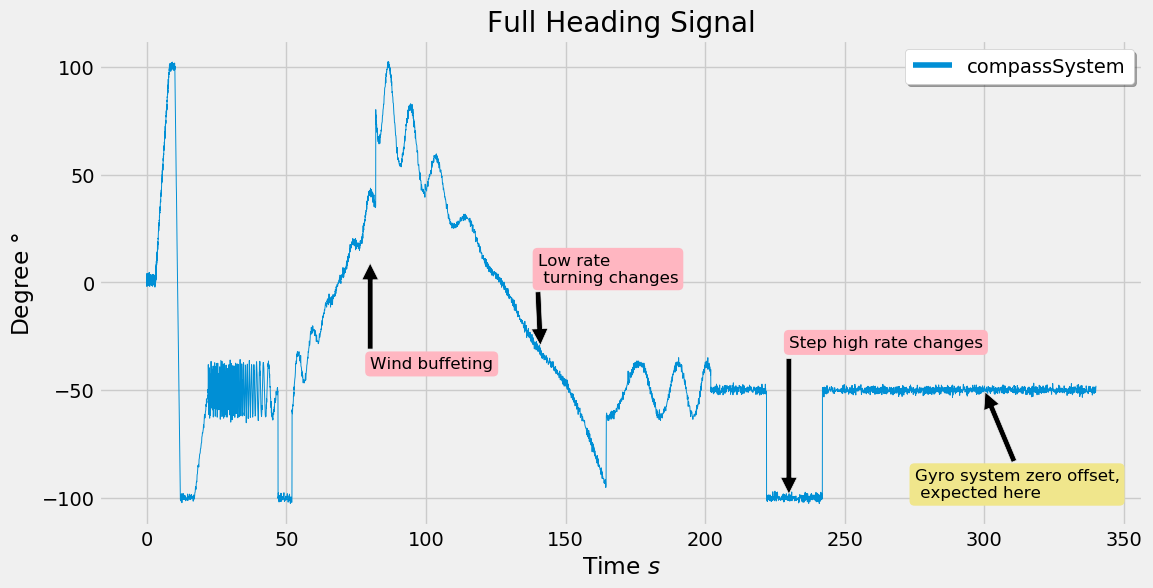
\includegraphics[width=\linewidth]{img/fullHeadingSignal.png}
    \caption{Complete heading signal.}
    \label{fig:raw_heading_signal}
\end{figure}

\begin{figure}[h]
    \centering
    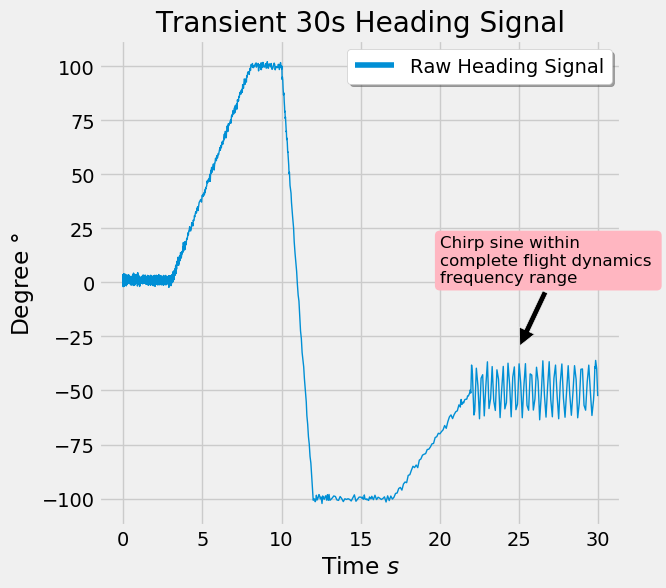
\includegraphics[width=0.75\linewidth]{img/headingSignal30s.png}
    \caption{Initial 30s of the heading signal.}
    \label{fig:transient_heading_signal}
\end{figure}

The heading signal can be separated into two analysis sections. From seconds 0 to 70, higher frequency changes aim to describe the transient response at the very limit of the DJI Mavic 2 physical operation. Part of this region is illustrated in Figure \ref{fig:transient_heading_signal}, although zoomed in to provide more detail. Drastic changes from 100 to -100 degrees are observed in a space of 3 seconds at the start, close to the rated turning rate of the DJI Mavic of 200 $\frac{\degree}{s}$. Random noise jitter with a mean of 0.05 $\degree$ has been added to the complete heading siganl to the minor imperfections in directional flight as can be individually noticed within the step signal or straight flight towards the end. The chirp sinusoidal wave between seconds 22 to 47 decreases frequency from 20 Hz to 0.01 Hz, within the range of most flight dynamics vibrations suggested by \cite{dorobantu2011frequency}. Mainly steep change slopes are observed at seconds 10, 20, 47 and 52 aim to demonstrate high rate turns.

The second section aims to test slower changes from second 70 onwards. Low rate turns with wind buffeting is described between seconds 50 to 120. Between seconds 160 and 210, sinusoidal waves also aim to demonstrate further low frequency behaviour. The rate gyro zero offset is expected to be observed towards the straight end of the heading flight.

During the design of the heading signal, several standard input signals such as the saw-tooth, sine, step, and delta waves with varying frequencies were independently inputted to understand the specific response of the system and design the heading signal for several frequency behaviours. Most of these independent signal responses are displayed within this heading signal.


\section{Results Analysis}

Multidimensional data analysis was performed to determine accurate statistical metrics to optimize the sensor fusion design. A set of signals comrpised of the raw time signals of the compass system, compass filter, full system combined, gyro system, gyro filter, and input heading signal can be observed in Figure \ref{fig:raw_time_signals_full}. In order to quantify the error of each sensor system output, the difference $\delta_k$ was determined for each signal $y_k$ with the input heading signal $y_i$. A set of new sensor data was created compounding by these differences $\delta_n$. To adequately quantify the error of each sensor output, analysis must be performed throughout a range of cutoff frequencies since this could drastically change the response of the full system. It is not expected that the independent system outputs for the gyro and compass systems would change over a range of cutoff frequencies since they are decoupled from this variation. However, the filter's response and full system response would change since they depend on the cutoff frequencies. Before describing the data analysis performed, the time responses of the signal's response to the heading input is observed in Figures \ref{fig:raw_time_signals_full} to \ref{fig:raw_error_signals_transient} for a 350 second simulation.

\begin{figure}[H]
    \centering
    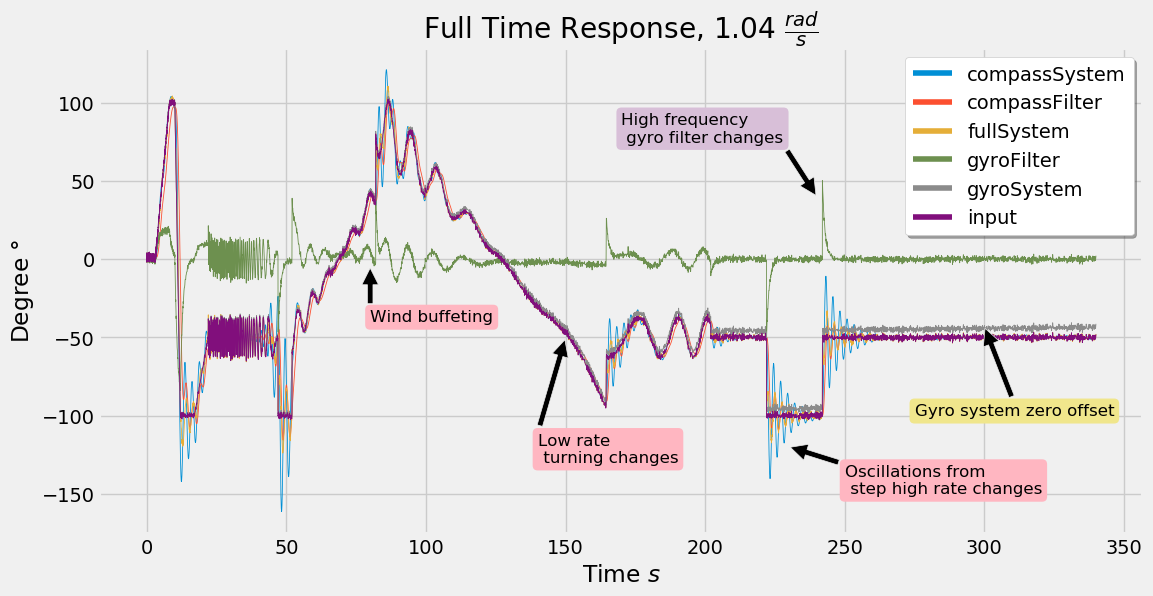
\includegraphics[width=\linewidth]{img/allSignalsFullTimeResponse_1_0476.png}
    \caption{All signals response to the heading input signal.}
    \label{fig:raw_time_signals_full}
\end{figure}

From Figure \ref{fig:raw_time_errors_full} it can be noticed that the full system error is considerably smaller than the error of each individual sensor due to the complementary filters. It can even be noticed that at very high frequencies such as near second 50, even the gyro filter begins oscillating potentially due to magnitude attenuation described in Figure \ref{fig:gyro_bode}.

The gyro filter output error mostly trails the inverse of the full system response in Figure \ref{fig:raw_time_errors_full}. At most points within the heading flight, the gyro filter output value in Figure \ref{fig:raw_time_signals_full} is near zero. Its magnitude suddenly increases to respond to higher frequency changes such as observed by the 40s chirp sine, 100s wind buffeting, 175s turning rates, or 225s step changes. This is expected due to the complementary filter mechanism that transfers all higher frequency excitation above the modelled 1.04 $\frac{rad}{s}$ cutoff frequency.

\begin{figure}[H]
    \centering
    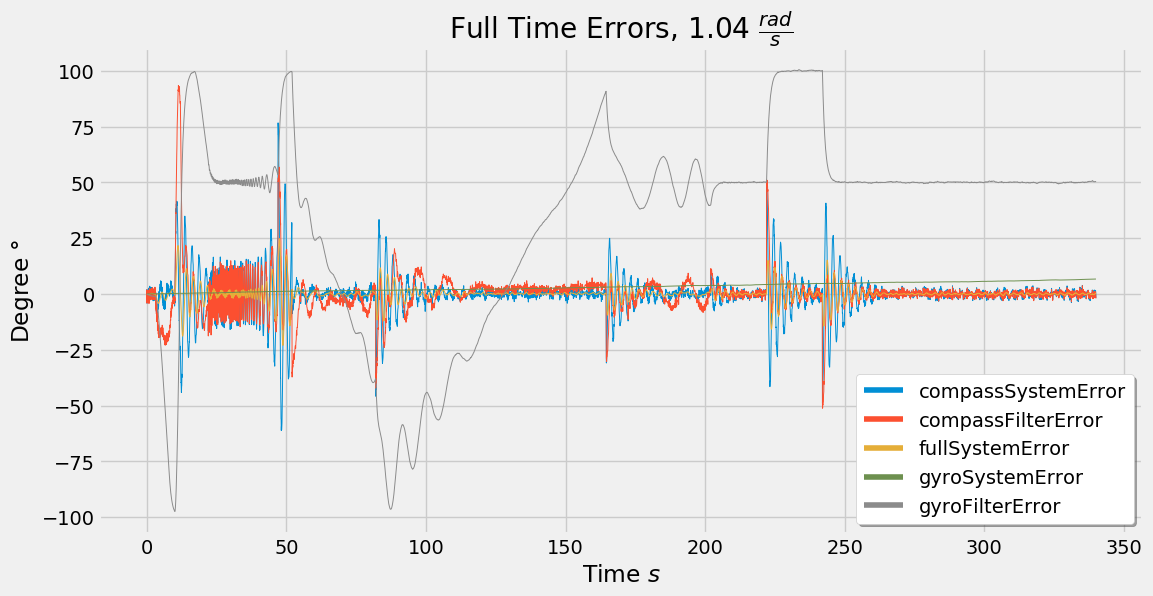
\includegraphics[width=\linewidth]{img/errorSignalsFullTimeResponse_1_0476.png}
    \caption{Error difference of each system signal for the full input heading signal.}
    \label{fig:raw_time_errors_full}
\end{figure}

The gyro system's zero offset from mechanical flight imperfections can be observed around 300 s, although for longer simulations that were run, it continuously increased which meant that high frequency oscillations were not accurately captured.

The compass filter and compass system trail the full system response at low frequencies, and these sensors oscillate at high frequency changes as observed in time 10s in Figure \ref{fig:raw_time_signals_transient}. Note that the full system oscillations are much lower since the complementary filter design compensates at high frequencies and reduces the compass system input into the response.

\begin{figure}[H]
\centering
\begin{subfigure}{0.495\textwidth}
  \centering
  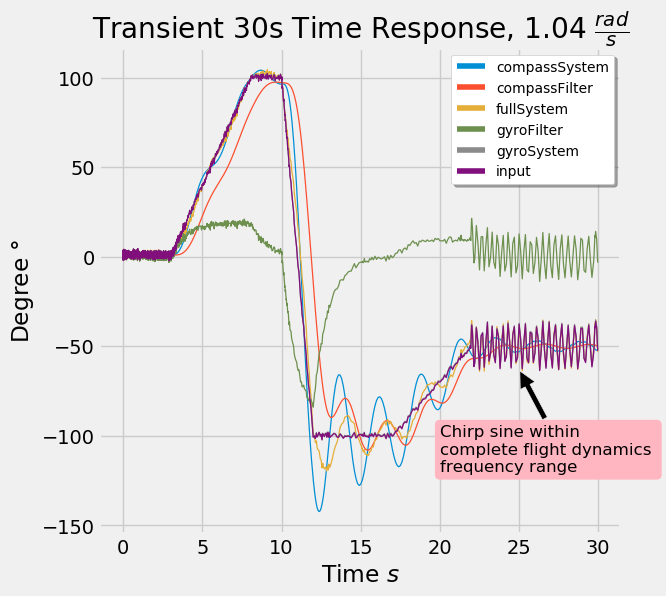
\includegraphics[width=\linewidth]{img/allSignalsTimeResponse30s_1_0476.png}
  \caption{Initial 30s response of all system signals. Note that the \texttt{input} legend refers to the heading signal.}
  \label{fig:raw_time_signals_transient}
\end{subfigure}
\begin{subfigure}{0.495\textwidth}
  \centering
  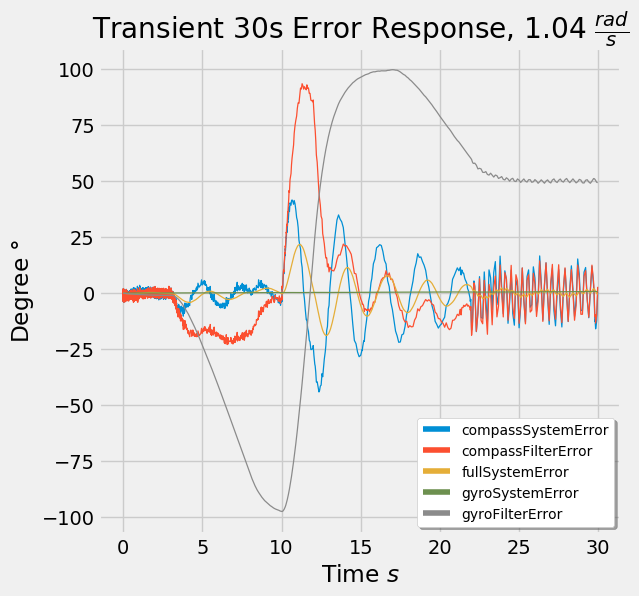
\includegraphics[width=\linewidth]{img/errorSignalsTimeResponse30s_1_0476.png}
  \caption{Error with the heading input of all the system signals. Note that the \texttt{input} legend refers to the heading signal.}
  \label{fig:raw_error_signals_transient}
\end{subfigure}
\caption{All signals initial 30s response.}
\end{figure}




\section{Error Quantification \&  Cutoff Frequency Variations}

The cutoff frequency was then varied within a frequency range of $10^{-2}$ to $10^2$ $\frac{rad}{s}$ and the above statistics were generated for all of them as described in Appendix \ref{sec:cutoff_error_variation_code}. With the aim of characterizing the error of each sensor output, the statistical analysis was mainly interested in seeing the point where the full system signal error is minimal. However, varying the simulation time changed this optimal value. Hence, futher analysis was done to practically determine the practical optimal cutoff frequency.

Since multidimensional data needed to be analysed, the Pandas Python data science package was used alongside Matplotlib 3D. Note that within the following analysis, exact values are always given since the random noise inputted in each heading signal simulation changes does not provide an identical response, but overall value ranges are noticed. This was done for the accuracy of attempting a real world heading signal simulation.

The three main sensor outputs that vary with the cutoff frequency are the gyro filter, compass filter and full system accordingly. Figures \ref{fig:full_system_cutoff_frequency} to \ref{fig:compass_filter_error_cutoff_frequency} describe provide a 3D plot representing how the time response and respective errors change with the variation of cutoff frequency. Whilst making the figures, a small section of the varied cutoff frequencies was selected to specifically demonstrate the changing behaviour. Figure \ref{fig:full_system_cutoff_frequency} shows how the overall time response of the full system varies. Within the range of 0 to 1.75 $rad/s$, it can be observed how response oscillations increase by comparing the initial amplitude of the time response to the final amplitude. To visualize this clearer, Figure \ref{fig:full_system_error_cutoff_frequency} demonstrates the difference between the full response and the input heading within a larger cutoff frequency range and the increase is noticeable. This is expected since it would mean that the compass, whose bode plot starts becoming nonlinear between 1 and 2 $rad/s$, begins responding to higher frequency oscillations.

% Full System vs Cutoff Frequency
\begin{figure}[H]
\centering
\begin{subfigure}{0.5\linewidth}
  \centering
  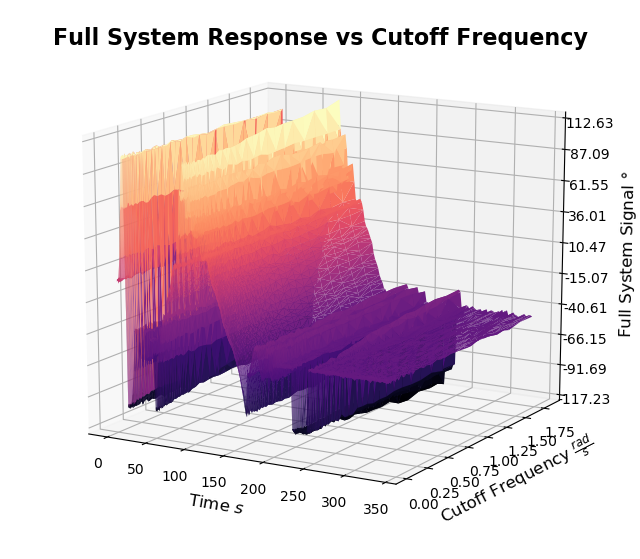
\includegraphics[width=\linewidth]{img/fullSystemCutoffFrequency.png}
  \caption{Full system amplitude time response vs cutoff frequency.}
  \label{fig:full_system_cutoff_frequency}
\end{subfigure}%
\begin{subfigure}{0.5\linewidth}
  \centering
  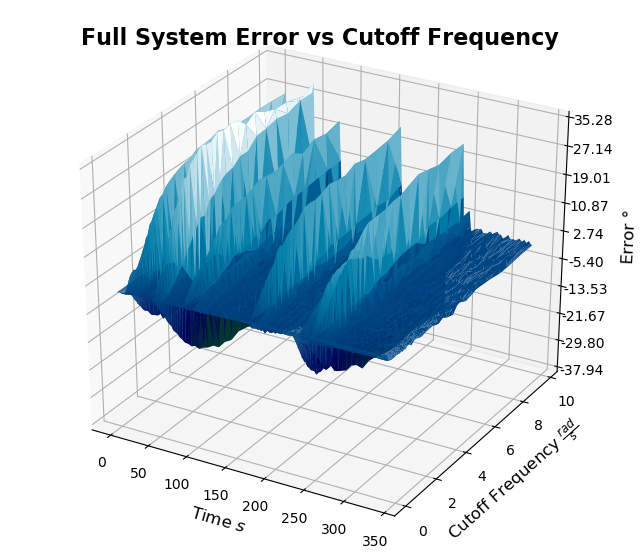
\includegraphics[width=\linewidth]{img/fullSystemErrorCutoffFrequency.png}
  \caption{Full system error variation in time}
  \label{fig:sub2}
\end{subfigure}
\caption{Full system error time response vs cutoff frequency. Note the difference in scales to adequately represent changes.}
\label{fig:full_system_error_cutoff_frequency}
\end{figure}

Figure \ref{fig:gyro_filter_error_cutoff_frequency} also demonstrates an interesting behaviour within a small cutoff frequency range of 0 to 1.75 $rad/s$. The gyro filter error response magnitude reaches steady state from 1.75 $rad/s$ to the rest of the cutoff frequencies, which is why only this range was modelled. The transient variation of the magnitude of the error in this graph within 0 and 1.25 $rad/s$ could be considered as differential change due to cutoff frequency change in the form $\frac{d(GyroEror)}{d(CutoffFrequency)}$. The steady state value is reached around 1 $rad/s$, and from this point on-wards the $\frac{d(GyroEror)}{d(CutoffFrequency)} \approx 0$. Considering this as a uni-variate optimization problem, it could be said that this is the optimal cutoff point since the compass is designed to operate adequately at lower frequencies. Also observing Figure \ref{fig:compass_filter_error_cutoff_frequency}, a 1 $rad/s$ compass cutoff frequency has relatively low error values in comparison to the rest of its error magnitude response after exponentially decreasing from a maximum near 0 $rad/s$. Hence, even in 3D space, the behaviour of complementary filter errors are demonstrated also when steady state values are reached. However, to fully discuss this, statistical time domain analysis needs to be performed.

% Gyro  and Compass Cutoff Filters over time
\begin{figure}[H]
\centering
\begin{subfigure}{0.5\linewidth}
  \centering
  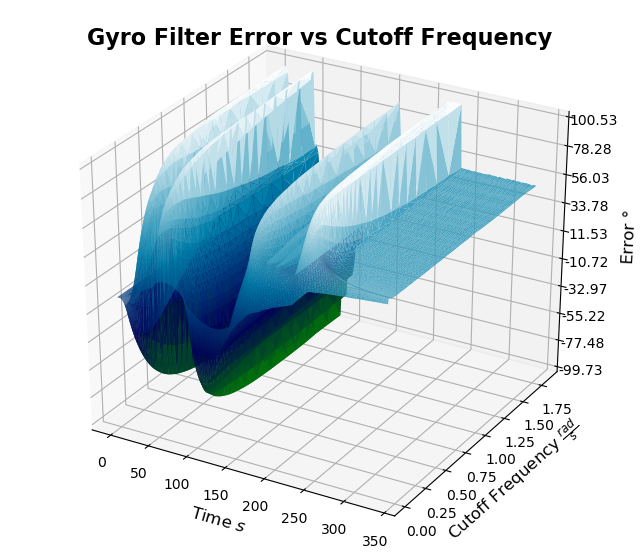
\includegraphics[width=\linewidth]{img/gyroFilterErrorCutoffFrequency.png}
  \caption{Gyro filter error variation with cutoff frequency over time.}
  \label{fig:gyro_filter_error_cutoff_frequency}
\end{subfigure}%
\begin{subfigure}{0.5\linewidth}
  \centering
  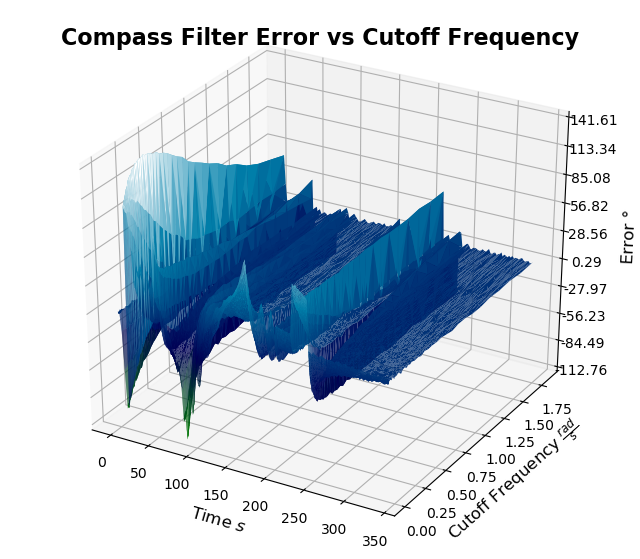
\includegraphics[width=\linewidth]{img/compassFilterErrorCutoffFrequency.png}
  \caption{Compass filter error variation with cutoff frequency over time.}
  \label{fig:sub2}
\end{subfigure}
\caption{Compass filter error variation with cutoff frequency over time.}
\label{fig:compass_filter_error_cutoff_frequency}
\end{figure}

% Carque et al. \cite{carque2011sensor} and Pasocal et al. \cite{pascoal2000navigation} demonstrate the accuracy benefits of sensor fusion
% ➢ T5.4 Propose a metric and quantify the error for each sensor output and for the fused output over the whole simulated flight. Hint – you may want to review the time domain statistical measures lecture. (10 marks)
A statistical metric cannot be chosen at random to quantify this error since all metrics provide different information about the signal data distribution. A comprehensive overall error metric might be a combination of different data statistics. In order to adequately select the error metric, or combined error metric, the following analysis were performed for both the raw signals and error sets: maximum, minimum, mean, standard deviation, variance, skewness, kurtosis, moments from 1 to 4, RMS, and 3dB power bandwidth (not for errors).  

Figures \ref{fig:sample_statistical_metrics} provides a sample of statistical metrics for all the signal errors whilst changing the cutoff frequency. In order to minimize the magnitude of the full system error, ideally its magnitude should be regularly near zero. However, realistically, because the incremental zero offset errors introduced into the gyro compass design that cannot be corrected via frequency filtering, the ideal value of the full system is when it matches the gyro system offset error within this model. It was noted that by varying the simulation time, the time-domain statistical optimal parameters vary; given the larger effect of the gyro system offset error. Hence, even if the time domain statistical parameters varied, what is required is selecting a cutoff frequency that is in steady state of the slope $\frac{d(SignalResponse)}{d(cutoffFrequency)} = 0$. At that point, the compass filter output is still at its maximum and the gyro filter output will have its standard zero-offset expected error. Hence, the response of the compass filters is not minimized specially when this is used to calibrate the gyro in flight during steady conditions. However, further time-domain statistical analysis will be performed in order to compare the optimal low statistic points for a specific simulation flight length with the steady cutoff frequency that is independent of this. This is because whilst the error magnitude may increase the overall zero offset rate is constant since it is not coupled mathematically as a function of the change of the cutoff frequency seen in Figure \ref{fig:full_system_error_cutoff_frequency}, only the filters are. 

The effect of varying cutoff frequencies on the amplitude of the response can be primarily observed in Figures \ref{fig:error_min} and \ref{fig:error_max}. If the cutoff frequency induces more oscillations, this will lead to larger differences within the response. It can be observed between the $10^{1}$ to $10^{2}$ regions that the full system response error stabilizes at a minima of around -60 and maxima of around 80. By the shape of the graphs, it can be inferred that oscillations differences are larger when the cutoff frequency is larger. This is expected since the compass filter would mainly respond to most flight oscillations, despite being optimized for lower frequencies.

The first aspect that will be analysed from the error differences are the standardized data moments which basically identify the crucial peak points within the data.

The mean ($\propto 1^{st} Moment$) is ${\rm}\mu ={\frac {1}{N}}\sum _{i=1}^{N}x_{i}.$ where $N$ is the time domain signal magnitude sample points. The mean is represented in Figure \ref{fig:error_mean}, but does not fully account for transient responses. However, it provides a general indication that the overall response averaged error $\frac{d(FullSystemEror)}{d(CutoffFrequency)}$ stabilizes to 0.1$\degree$ at a 0.13 $rad/s$. However, the mean has already reached a near zero value before the $10^{-1}$. Potentially because the system has not run for long enough, the mean is near 0 and has not stabilized yet to the gyro system error. It is also worth noting that there is a near-inflection point for both the compass (blue) and gyro (green) filter error plots at this point, which is related to a cutoff frequency change. Hence, the mean might not be an accurate error metric for the overall system error minimization response. % todo assume first moment

The standard deviation ($\propto 2^{nd} Moment$) for each cutoff frequency is $\sigma ={\sqrt {{\frac {1}{N}}\sum _{i=1}^{N}(x_{i}-\mu )^{2}}}$ where $X_i$ is a time domain sample point, and this illustrates how large the distribution of overall errors is from the averaged value in Figure \ref{fig:error_standard_deviation}. Hence, for a larger $\sigma$ is, it means that $X_i$ varied errors can be drastically different from the overall averaged error. It could also mean that oscillations could be very large but quick. When the objective is to minimize both transient and overall errors, it is desired that the overall error magnitude value and distribution of errors to be near zero. The full system has an minimum point where the distribution is near 0 at 0.048 $rad/s$. Again there appears to be an inflection point at this value for the compass and gyro filters. However, since it is known that practically that minimum is not the ideal value due to the increasing zero-offset observed during large simulation times, it can also be observed that at about 1 $rad/s$ the gyro filter error and compass filter errors reach a steady state value. The full system plot intersects also with the gyro system error plot. This was expected from observing their time responses in Figure \ref{fig:compass_filter_error_cutoff_frequency}.

Again regarding the full system signal, the skewness ($\propto 3^{nd} Moment$) and kurtosis ($\propto 4^{th} Moment$) in Figures \ref{fig:error_skewness} \& \ref{fig:error_kurtosis}  provide understanding of the asymmetrical accentuation of the probabilistic distribution of data around a overall mean value. The interesting aspect is that both signals have a maximum at the values around 0.048 $rad/s$. They also seem to reach steady state values slightly before or after $10^1$ $rad/s$ as expected from previous moments.

When characterizing the gyro system error, it is known that there will be zero offset as mechanical forces destabilize it during the heading flight. At its latest position, it has a $8.66 \degree$ difference for 350s heading flight. Assuming a linear slope, this offset error will only increase with longer flights, its slope in this simulation is $\approx 0.025 \degree/s = \approx 1.5 \degree/min$ as seen in Figure \ref{fig:raw_time_signals_full} which validates our design goal. Its standard deviation remains constant around 2.13 since the only changes are from a few high frequency turning rates that lead to higher errors (as observed) in Figure \ref{fig:raw_time_errors_full}.

The root mean squared RMS of a function $g(t)$ is ${\displaystyle g_{\text{RMS}}=\lim _{T\rightarrow \infty }{\sqrt {{1 \over {T}}{\int _{0}^{T}{[g(t)]}^{2}\,dt}}}.}$ where $T$ is the number of sample points of the response function $g(t)$. Because the mean of all the squared magnitudes of the signal are considered, it provides a general indication of the ``energy" value of the wave. It can also be noted that there is a minima around 0.048 $rad/s$. This full system error has an inflection point around 1 $rad/s$ where it intersects with the gyro system error probably due to the inverse stabilization of the the gyro and compass filter magnitudes.

Hence, an error metric for each sensor is required to be derived. It is known that the RMS and standard deviation are the most accurate statistics to determine the optimal cutoff frequency at the intersection of the gyro system error and the full system error. The error with any other cut-off frequency can be determined by the absolute difference between the full system error and gyro system error accordingly. Also, because the gyro filter and compass filter behave nearly inversely, as in Figure \ref{fig:error_standard_deviation}, the difference between the two can be compared to an optimal difference in magnitude of 32.52 for the standard deviation and 37.63 for the RMS. Since there is an inflection point for both error signals, this can be related to the ideal minimum for that specific flight time and this point will move towards the right as the flight time is increased. Hence, a geometrical relationship can be derived from these graphs. Integrating this analysis together constraining it to give a value between 0 and unity of error can be written in Equation \ref{eq:error_metic}, where $E_m$ is the error metric, $\Delta\sigma$ is the difference in the standard deviation for that cut-off frequency $w_c$, and $\Delta\kappa$ is the difference in RMS values. The closer it is to 0, the cutoff frequency is closer to the ideal one.

\begin{equation}
    E_m(w_c) = \frac{32.52\Delta\Sigma}{37.63} + \frac{37.63 \Delta\kappa}{32.52}
    \label{eq:error_metic}
\end{equation}

This metric can be compared to different heading flights and possibly the ideal difference values can be calibrated after testing over a further range of frequencies and simulation time. In summary, multi-dimensional Big Data time statistical analysis was used to determine the optimal design parameters of a sensor fusion system.

\begin{figure}[H]
 % First
\begin{subfigure}{.5\textwidth}
  \centering
  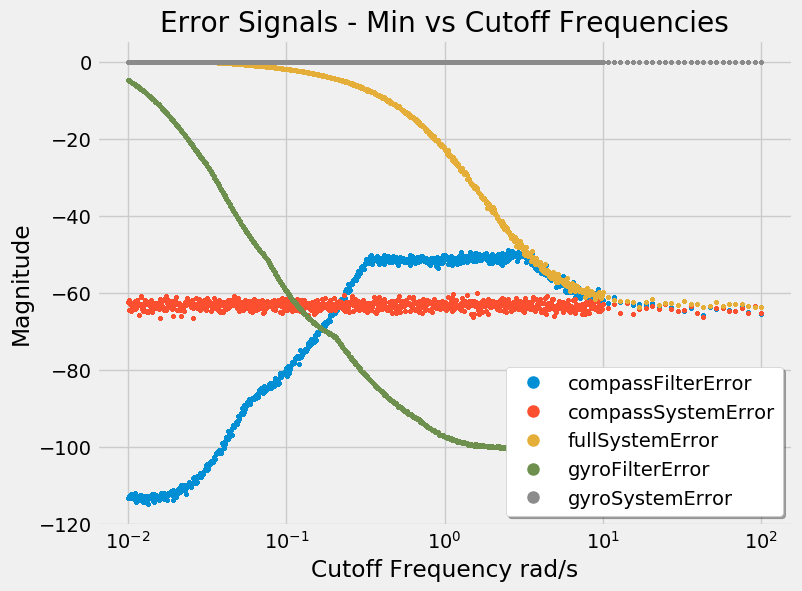
\includegraphics[width=\linewidth, height=\paperheight/5]{img/iterable/errorsSignals/errorminSignals.png}  
  \caption{Signal errors minimum value.}
  \label{fig:error_min}
\end{subfigure}
% Second
\begin{subfigure}{.5\textwidth}
  \centering
  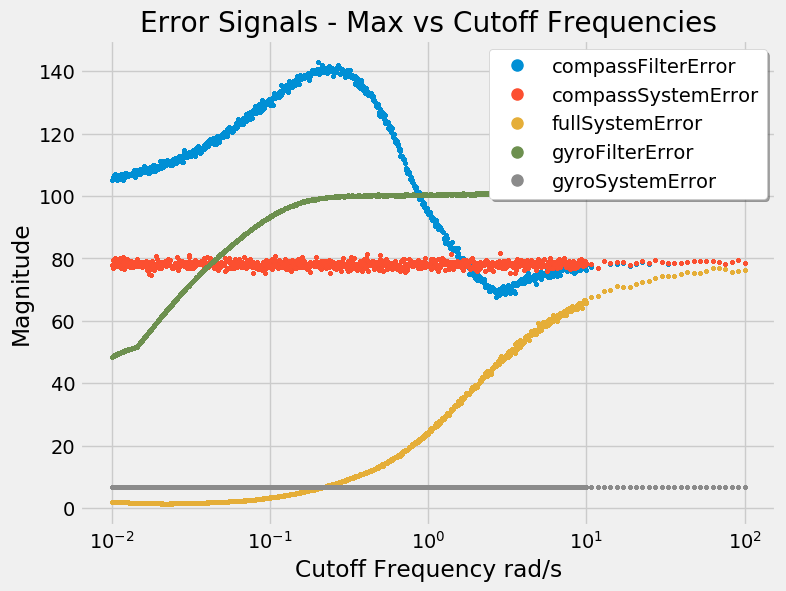
\includegraphics[width=\linewidth, height=\paperheight/5]{img/iterable/errorsSignals/errormaxSignals.png} 
  \caption{Signal errors maximum value.}
  \label{fig:error_max}
\end{subfigure}
% Third
\begin{subfigure}{.5\textwidth}
\centering
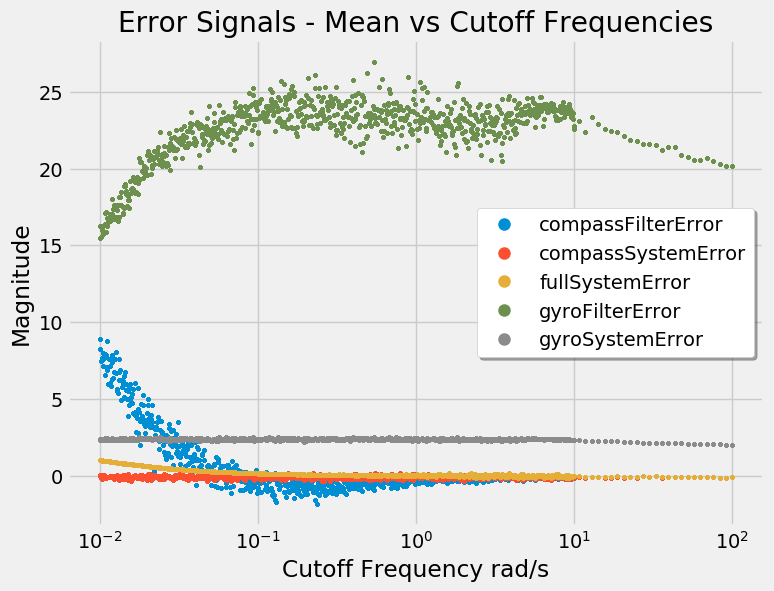
\includegraphics[width=\linewidth, height=\paperheight/5]{img/iterable/errorsSignals/errormeanSignals.png}  
  \caption{Signal errors mean value ($\propto1^{st}$ Moment)}
\label{fig:error_mean}
\end{subfigure}
  % Fourth
\begin{subfigure}{.5\textwidth}
  \centering
  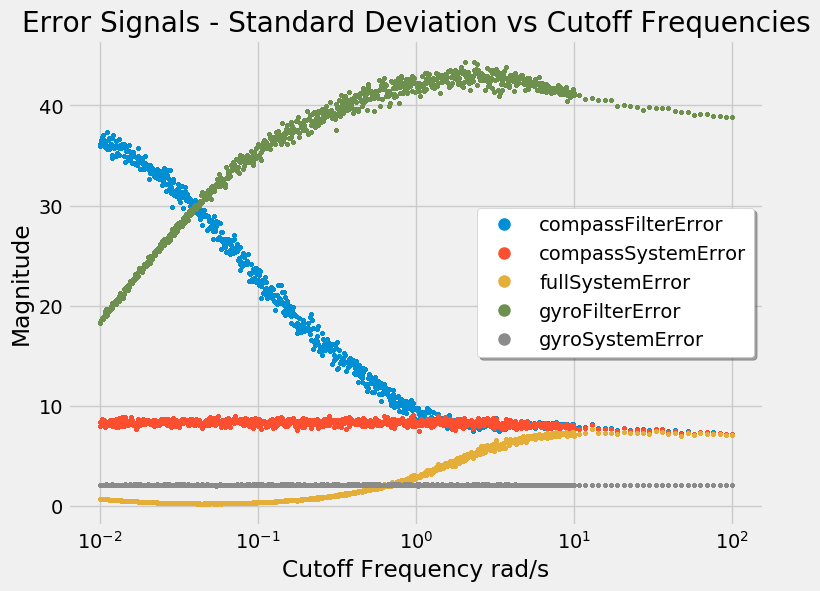
\includegraphics[width=\linewidth, height=\paperheight/5]{img/iterable/errorsSignals/errorstandardDeviationSignals.png}  
  \caption{Signal errors standard deviation. ($\propto2^{nd}$ Moment)}
  \label{fig:error_standard_deviation}
\end{subfigure}
% Fifth
\begin{subfigure}{.5\textwidth}
  \centering
  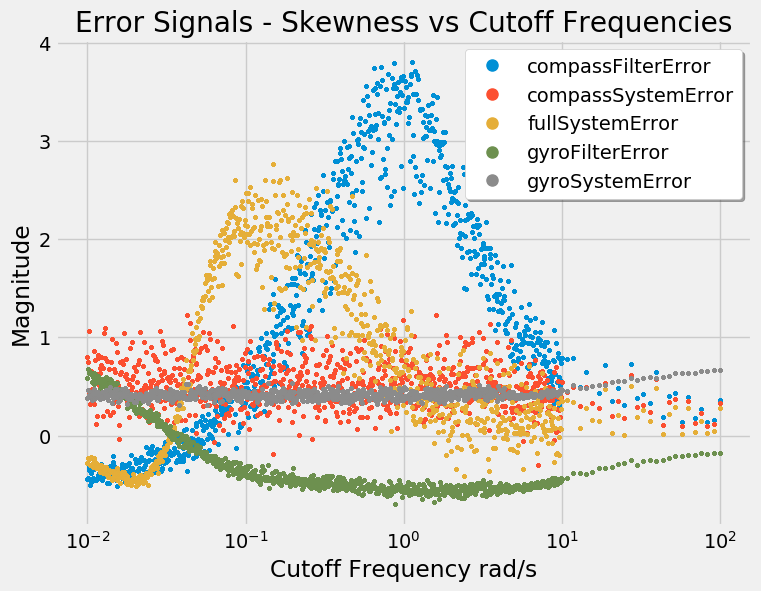
\includegraphics[width=\linewidth, height=\paperheight/5]{img/iterable/errorsSignals/errorskewnessSignals.png}  
  \caption{Signal errors skewness. ($\propto3^{rd}$ Moment)}
  \label{fig:error_skewness}
\end{subfigure}
  % Sixth
\begin{subfigure}{.5\textwidth}
  \centering
  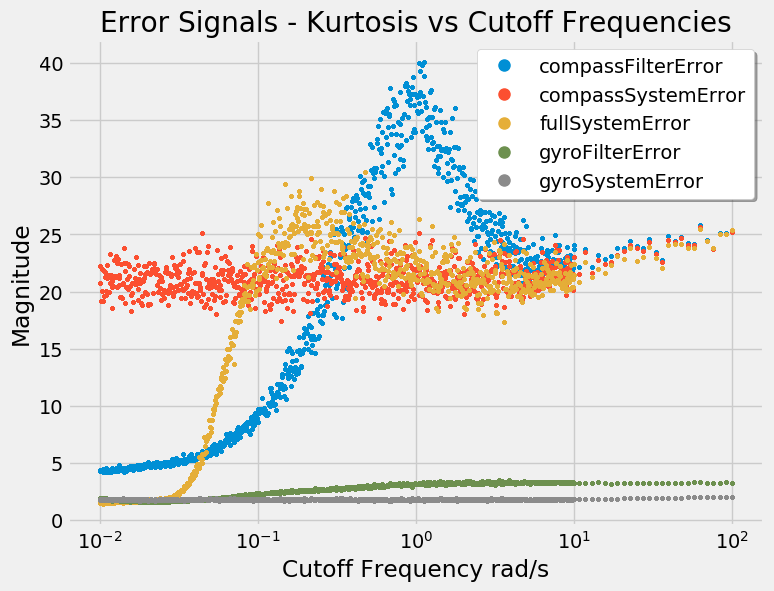
\includegraphics[width=\linewidth, height=\paperheight/5]{img/iterable/errorsSignals/errorkurtosisSignals.png}  
  \caption{Signal errors kurtosis ($\propto4^{th}$ Moment)}
  \label{fig:error_kurtosis}
\end{subfigure}
% Seventh
\begin{subfigure}{.5\textwidth}
  \centering
  % Eigth
  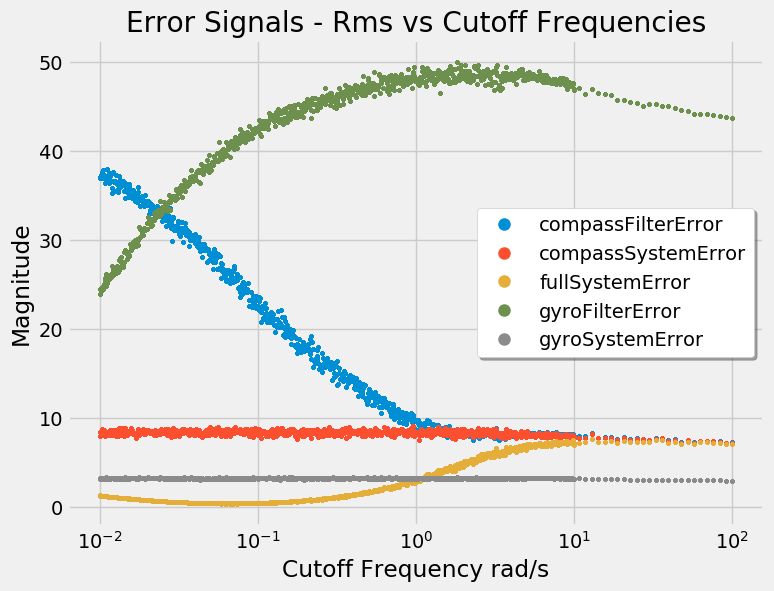
\includegraphics[width=\linewidth, height=\paperheight/5]{img/iterable/errorsSignals/errorrmsSignals.png}  
  \caption{Signal error RMS (Energy).}
  \label{fig:error_rms}
\end{subfigure}
\caption{Error differences with cutoff frequencies}
\label{fig:sample_statistical_metrics}
\end{figure}




% https://tex.stackexchange.com/questions/53458/inserting-figures-using-loops

% \section{Cutoff Frequency Variations}
% ➢ T5.5 Explore how variations in the True Heading Signal or in the filter cut-off frequency affect the measured error. (10 marks) 

\printbibliography

\appendix
\section{Appendix}

\subsection{Signals Time Domain Statistical Analysis}
\begin{figure}[H]
 % First
\begin{subfigure}{.5\textwidth}
  \centering
  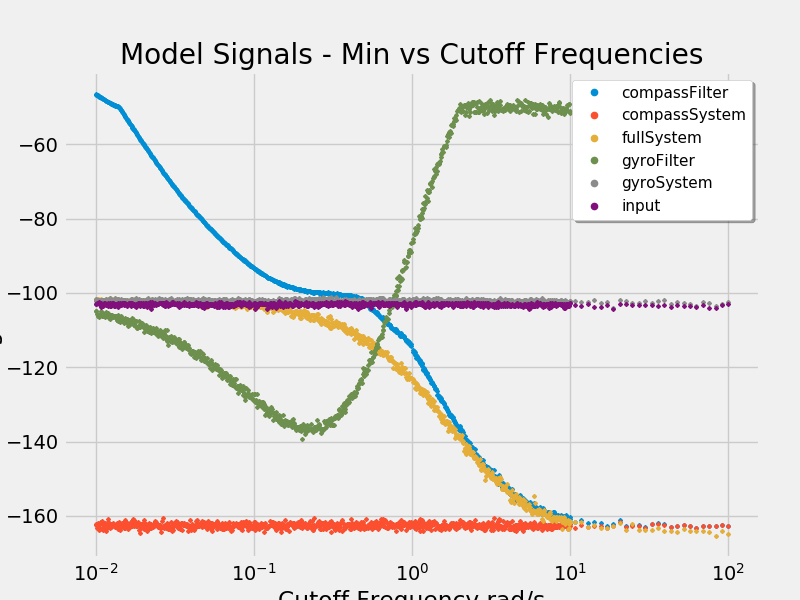
\includegraphics[width=\linewidth, height=\paperheight/5]{img/iterable/modelSignals/modelminSignals.png}  
  \caption{Signals minimum value.}
  \label{fig:model_min}
\end{subfigure}
% Second
\begin{subfigure}{.5\textwidth}
  \centering
  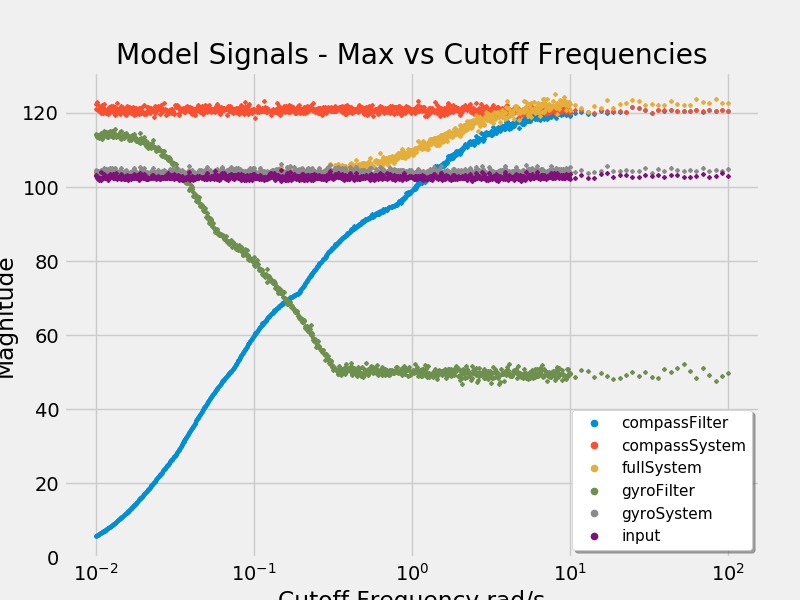
\includegraphics[width=\linewidth, height=\paperheight/5]{img/iterable/modelSignals/modelmaxSignals.png} 
  \caption{Signals maximum value.}
  \label{fig:model_max}
\end{subfigure}
% Third
\begin{subfigure}{.5\textwidth}
\centering
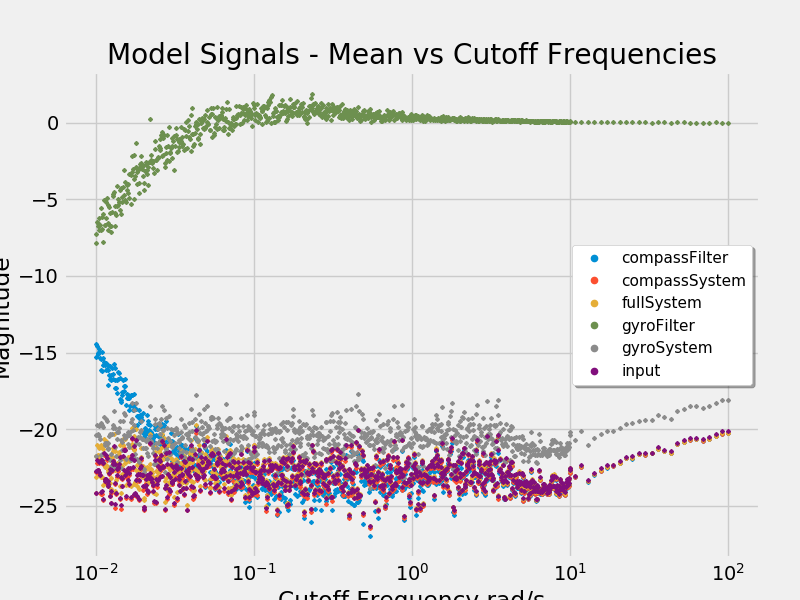
\includegraphics[width=\linewidth, height=\paperheight/5]{img/iterable/modelSignals/modelmeanSignals.png}  
  \caption{Signals mean value ($\propto1^{st}$ Moment)}
\label{fig:model_mean}
\end{subfigure}
  % Fourth
\begin{subfigure}{.5\textwidth}
  \centering
  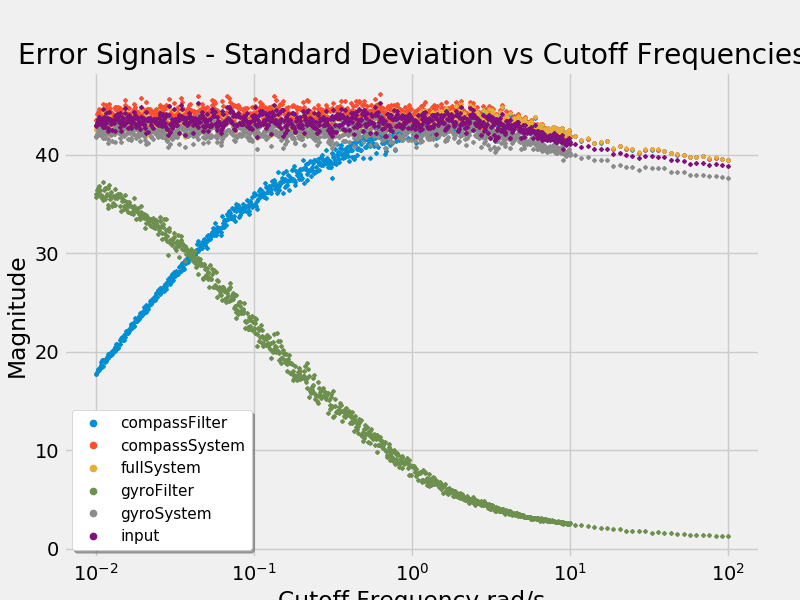
\includegraphics[width=\linewidth, height=\paperheight/5]{img/iterable/modelSignals/modelstandardDeviationSignals.png}  
  \caption{Signals standard deviation. ($\propto2^{nd}$ Moment)}
  \label{fig:model_standard_deviation}
\end{subfigure}
% Fifth
\begin{subfigure}{.5\textwidth}
  \centering
  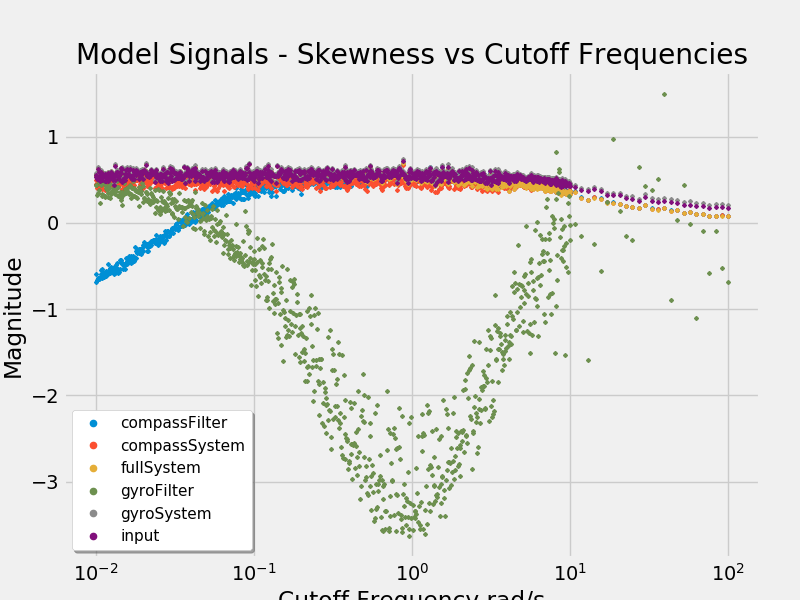
\includegraphics[width=\linewidth, height=\paperheight/5]{img/iterable/modelSignals/modelskewnessSignals.png}  
  \caption{Signals skewness. ($\propto3^{rd}$ Moment)}
  \label{fig:model_skewness}
\end{subfigure}
  % Sixth
\begin{subfigure}{.5\textwidth}
  \centering
  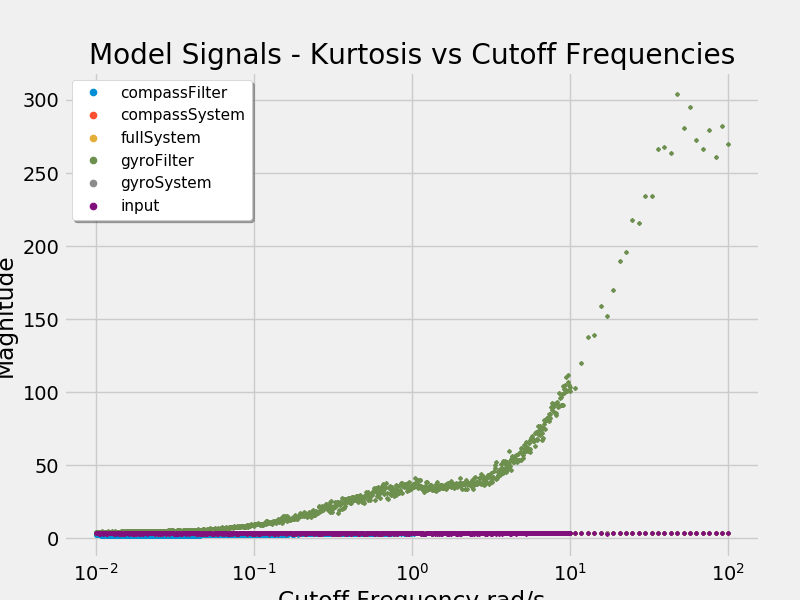
\includegraphics[width=\linewidth, height=\paperheight/5]{img/iterable/modelSignals/modelkurtosisSignals.png}  
  \caption{Signals kurtosis ($\propto4^{th}$ Moment)}
  \label{fig:model_kurtosis}
\end{subfigure}
% Seventh
\begin{subfigure}{.5\textwidth}
  \centering
  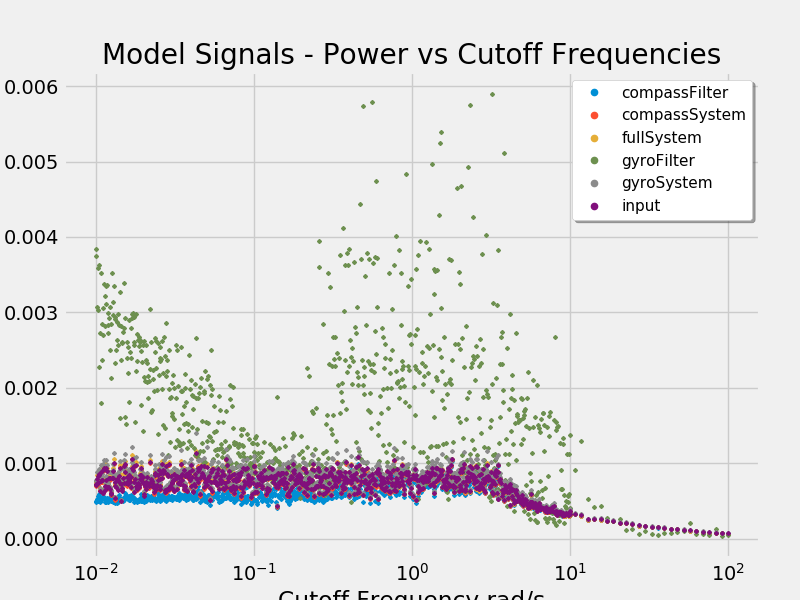
\includegraphics[width=\linewidth, height=\paperheight/5]{img/iterable/modelSignals/modelpowerSignals.png}  
  \caption{Signals 3dB power bandwidth}
  \label{fig:model_power}
\end{subfigure}
\begin{subfigure}{.5\textwidth}
  \centering
  % Eigth
  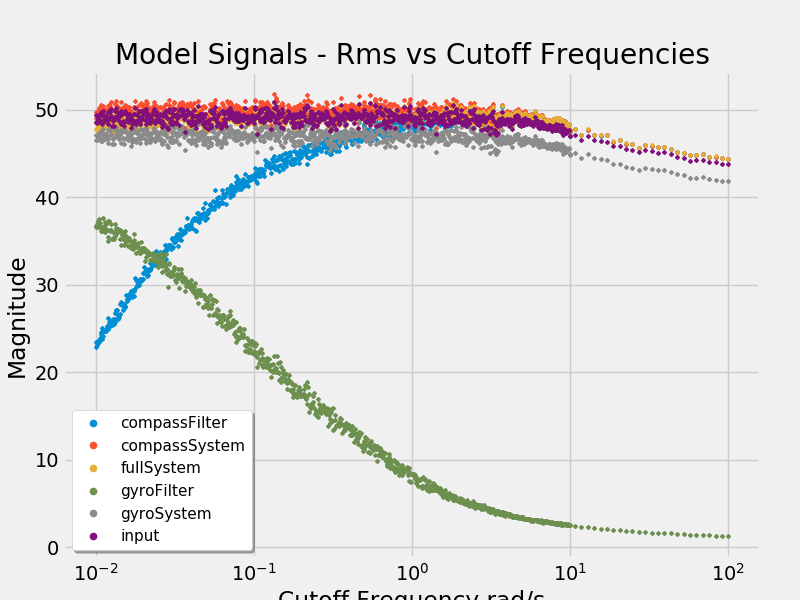
\includegraphics[width=\linewidth, height=\paperheight/5]{img/iterable/modelSignals/modelrmsSignals.png}  
  \caption{Signals RMS (Energy)}
  \label{fig:model_rms}
\end{subfigure}
\caption{Signals time-domain statistical analysis.}
\label{fig:sample_statistical_metrics}
\end{figure}

\subsection{Cutoff Frequency Variation Code}
\label{sec:cutoff_error_variation_code}
\inputminted{octave}{code/errorCutoffFrequencyVariation.m}

\subsection{Heading Signal MATLAB System Block}
\label{sec:heading_signal_code}
\inputminted{octave}{code/HeadingSignals.m}



\end{document}
